\documentclass[a4paper,12pt]{article} 
\usepackage[top = 2.5cm, bottom = 2.5cm, left = 2.5cm, right = 2.5cm]{geometry} 
\usepackage[T1]{fontenc}
\usepackage{multirow} 
\usepackage{amsmath}
\usepackage{booktabs} 
\usepackage{amssymb}
\usepackage{graphicx} 
\usepackage{setspace}
\usepackage{float}
\usepackage{fancyhdr}
\usepackage{fancybox}
\usepackage{graphicx}
\usepackage{caption}
\usepackage{float}
\usepackage[framemethod=tikz]{mdframed}
\usetikzlibrary{shadows}

\newmdenv[shadow=true,shadowcolor=black,font=\sffamily,rightmargin=8pt]{shadedbox}


\pagestyle{fancy}

\fancyhf{}

\lhead{\footnotesize Inv. de Operaciones: Tarea Final}

\rhead{\footnotesize Martin Mancilla, Claudio Duran}

\cfoot{\footnotesize \thepage} 

\begin{document}
	
\thispagestyle{empty}

\begin{tabular}{p{15.5cm}}
	{\large \bf Investigación de Operaciones} \\
	Universidad Católica del Maule \\ 
	Martín Mancilla V. - Claudio Durán N.\\
	\textit{19.386.399-k} - \textit{19.215.697-1} \\
	\textit{https://github.com/Marmanvii/ilog-cplex-problems}\\
	\hline
	\\
\end{tabular}

\vspace*{0.3cm}

\begin{center}
	{\Large \bf TRABAJO FINAL} 
	\vspace{2mm}
	
	% YOUR NAMES GO HERE
	{Resolución de Problemas de Optimización}
	
\end{center}  

\vspace{0.4cm}

\section{Primer Problema}
\subsection{Formule  el  modelo  que  permita  obtener  el  portafolio de  inversión  que  optimice  el  retorno  esperado  de  la	corporación y simultáneamente no viole su política de inversión}
\subsubsection{Variable de Decisión}
\begin{equation*}
	\begin{split}
		N &= \{1,2,3,4,5\} \\
		X_i & = \text{Cantidad invertida en categoría } i \text{ de la inversión. } \forall i \in N
	\end{split}
\end{equation*}
\begin{center}
	\noindent\rule{12cm}{0.4pt}
\end{center}
\begin{shadedbox}
1 = Acciones comunes, 2 = Cuotas de fondos mutuos, 3 = Bonos de Oferta Pública,\\ 4 = Bonos de Gobierno, 5 = Cuentas de Ahorro
\end{shadedbox}
\subsubsection{Constantes}
\begin{equation*}
\begin{split}
	RAE &= [0.15,\ 0.12,\ 0.10,\ 0.05,\ 0.08] \\
	FR & = [1.6,\ 1.0,\ 0.5,\ 0.0,\ 0.1] \\
	RAE_i &= \text{ Retorno Anual Esperado para la categoría } i \text{ de la inversión } \forall i \in N. \\
	FR_i &= \text{Factor de riesgo para la categoría } i \text{ de la inversión } \forall i \in N.
\end{split}
\end{equation*}
\subsubsection{Función Objetivo}
\begin{equation*}
\begin{split}
	maxZ = \sum_{i = 1}^{5}X_i\times RAE_i
\end{split}
\end{equation*}
\subsubsection{Restricciones}
\begin{enumerate}
	\item La inversión en acciones y en cuotas de fondos mutuos no debe ser mayor que un
	30\% del total de  las  inversiones.
	\begin{equation*}
		x_1 + x_2 \leq 0.3\times\sum_{i = 1}^{5}x_i
	\end{equation*}
	\item La  inversión  en  bonos  de  gobierno  no  debe  ser  inferior  a  la  inversión  en  cuentas  de  ahorro.
	\begin{equation*}
		x_4 \geq x_5
	\end{equation*}
	\item La inversión en debentures y bonos de gobierno no debe exceder el 50\% del total de las inversiones.
	\begin{equation*}
		x_3 + x_4 \leq 0.5\times\sum_{i = 1}^{5}x_i
	\end{equation*}
	\item La inversión en bonos de gobierno debe superar el 25\% del total de las inversiones.
	\begin{equation*}
		x_4 \geq 0.25\times\sum_{i = 1}^{5}x_i
	\end{equation*}
	\item La corporación Gamma    requiere invertir  la  suma  de  US\$  1.000.000  en el  próximo  año  fiscal.
	\begin{equation*}
		\sum_{i = 1}^{5}x_i \leq 1,000,000
	\end{equation*} 
	\item La corporación  no  permite  que el  portafolio  de  valores  escogidos  tenga  un  factor de  riesgo ponderado mayor que 1.0.
	\begin{equation*}
		\sum_{i = 1}^{5}x_i\times FR_i \leq 1.0 \times \sum_{i = 1}^{5}x_i
	\end{equation*}
	\item No negatividad.
	\begin{equation*}
		x_i\geq 0\ \forall i \in N
	\end{equation*}
\end{enumerate}
\subsubsection{Valores óptimos y solución}
\begin{itemize}
	\item Soluciones óptimas:
	\begin{enumerate}
		\item $x_1=300000\text{ dólares}$
		\item $x_2=0\text{ dólares}$
		\item $x_3=250000\text{ dólares}$
		\item $x_4=250000\text{ dólares}$
		\item $x_5=200000\text{ dólares}$
	\end{enumerate}
\end{itemize}
$\therefore$ Valor óptimo: $z=98500 \text{ dólares}$
\newpage
\subsection{Comentarios}
\begin{figure}[H]
	\centering
	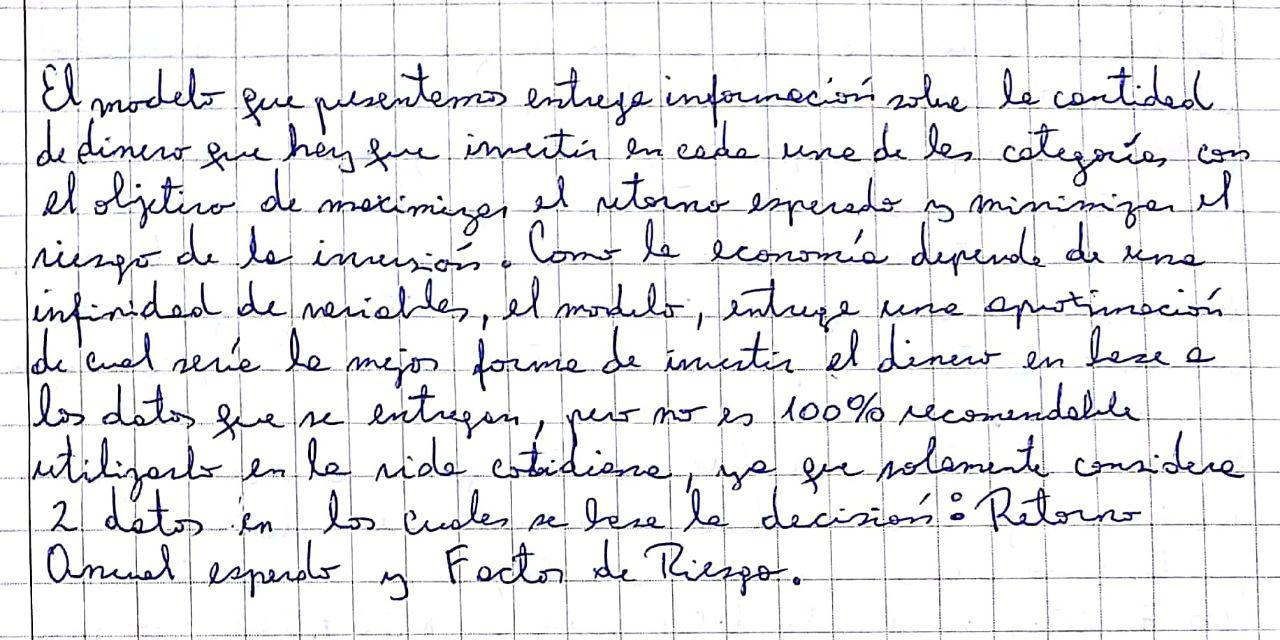
\includegraphics[scale=0.5]{claudio1.jpg}
	\caption*{Comentario de Claudio Durán}
\end{figure}
\begin{figure}[H]
	\centering
	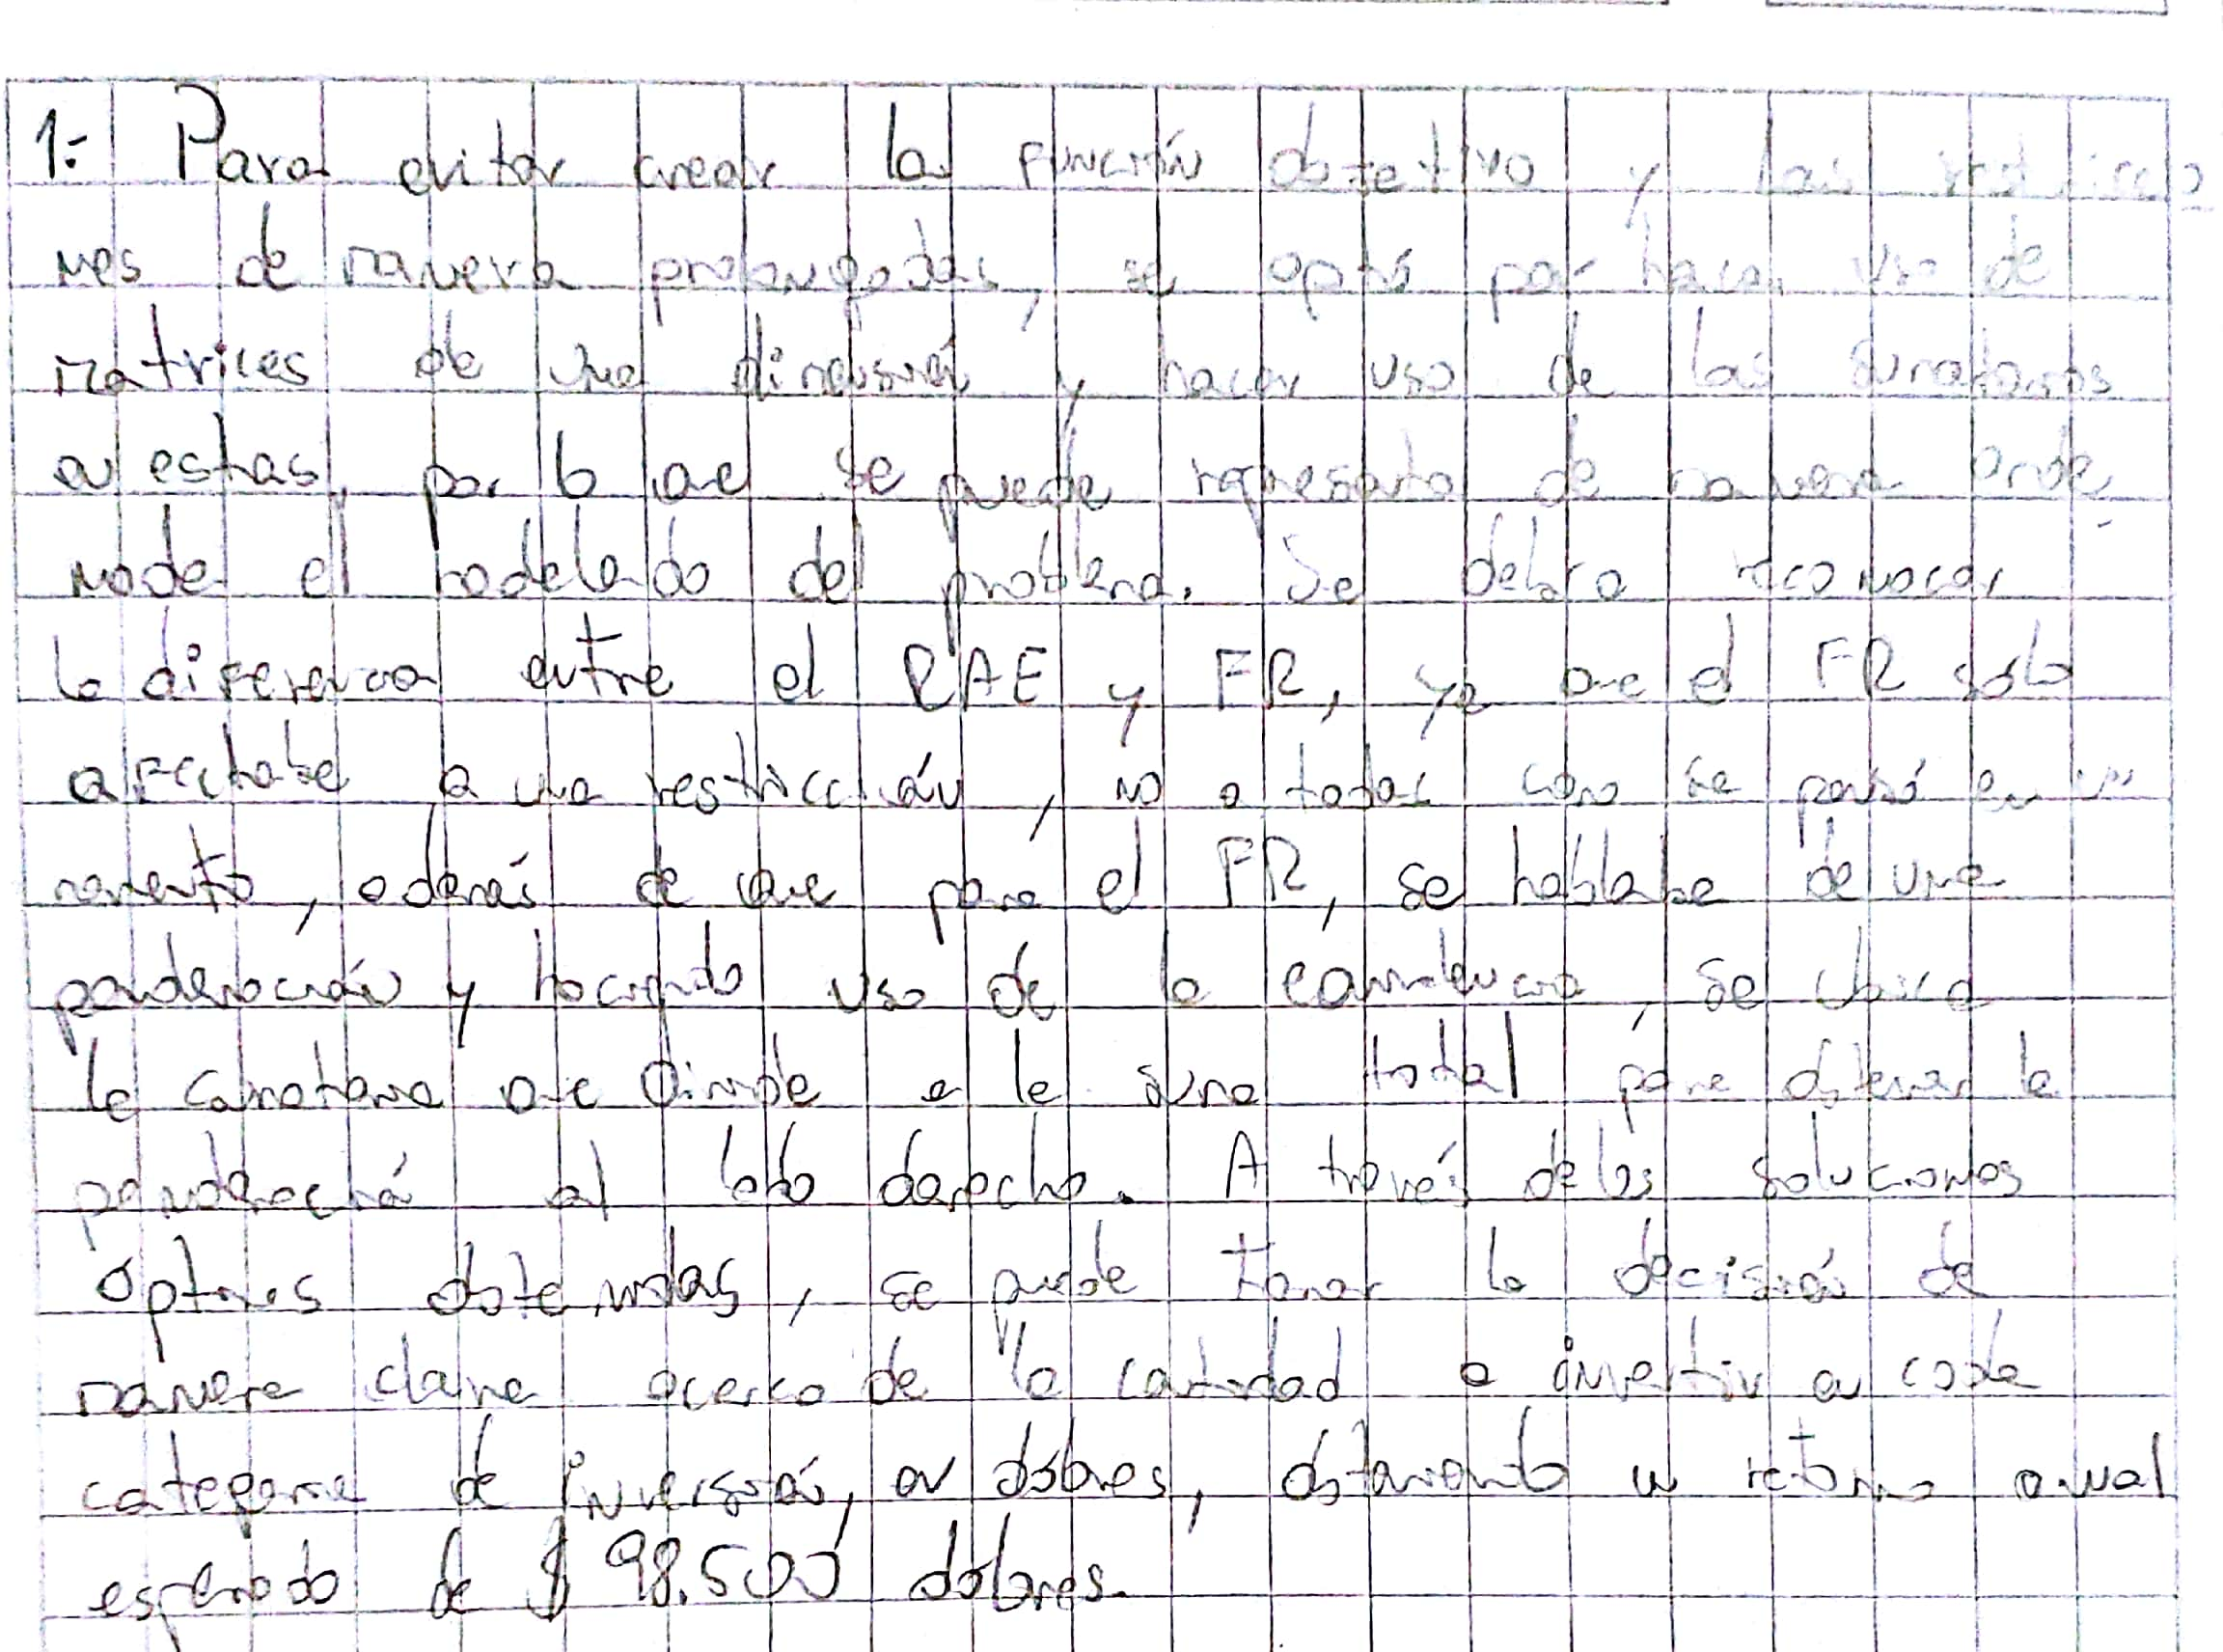
\includegraphics[scale=0.2]{martin1.jpg}
	\caption*{Comentario de Martin Mancilla}
\end{figure}
\newpage
\section{Segundo Problema}
\subsection{Dibuje el grafo que represente el problema.}
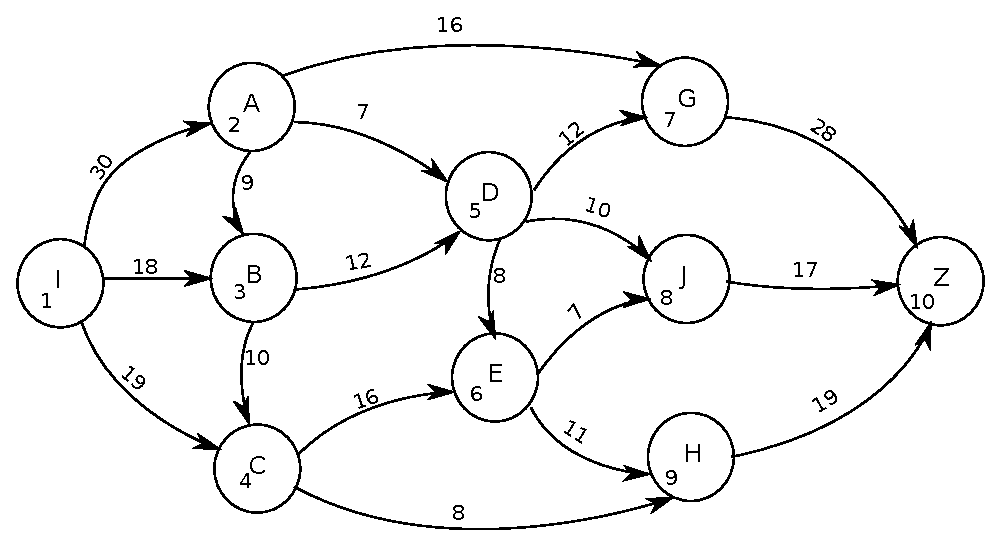
\includegraphics[scale=1]{drawing.eps}
\subsection{Formule el modelo que le permite resolver este problema}
\subsubsection{Nodos y Aristas}
\begin{equation*}
\begin{split}
	N = &\{1,2,3,4,5,6,7,8,9,10\} \\
	A = &\{ (1,2)(1,3)(1,4)(2,3)(2,5)(2,7)(3,4)(3,5)(4,6)\\
	  &(4,9)(5,6)(5,7)(5,8)(6,8)(6,9)(7,10)(8,10)(9,10) \}
\end{split}
\end{equation*}
\subsubsection{Variable de Decisión}
\begin{equation*}
\begin{split}
	X_{ij} &= \text{Cantidad de mensajes transmitidos de nodo } i \text{ a nodo } j \ (\forall(i,j)\in A)\\
	v &= \text{Flujo máximo de los nodos}
\end{split}
\end{equation*}

\subsubsection{Función Objetivo}
\begin{equation*}
	maxZ = v
\end{equation*}

\subsubsection{Restricciones}
\begin{itemize}
	\item Nodo Oferta
		\begin{equation*}
		\text{(1) }	X_{12}+X_{13}+X_{14}=v	
		\end{equation*}
	\item Nodo Demanda
		\begin{equation*}
		\text{(10)}	-X_{710}-X_{810}-X_{910}=-v
		\end{equation*}
	\item Nodos Transición
		\begin{equation*}
		\begin{split}
			\text{(2) }&X_{23}+X_{25}+X_{27}-X_{12}=0\\
			\text{(3) }&X_{34}+X_{35}-X_{13}-X_{23}=0\\
			\text{(4) }&X_{46}+X_{49}-X_{14}-X_{34}=0\\
			\text{(5) }&X_{56}+X_{57}+X_{58}-X_{25}-X_{35}=0\\
			\text{(6) }&X_{68}+X_{69}-X_{46}-X_{56}=0\\
			\text{(7) }&X_{710}-X_{27}-X_{57}=0\\
			\text{(8) }&X_{810}-X_{58}-X_{68}=0\\
			\text{(9) }&X_{910}-X_{49}-X_{69}=0
		\end{split}
		\end{equation*}
		\item Capacidad de aristas
		\begin{equation*}
		\begin{split}
			X_{12}&\leq 30 \qquad X_{34}\leq 10 \qquad X_{58}\leq 10\\
			X_{13}&\leq 18 \qquad X_{35}\leq 12 \qquad X_{68}\leq 7\\
			X_{14}&\leq 19 \qquad X_{46}\leq 16 \qquad X_{69}\leq 11\\
			X_{23}&\leq 9 \qquad X_{49}\leq 8 \qquad X_{710}\leq 28\\
			X_{25}&\leq 7 \qquad X_{56}\leq 8 \qquad X_{810}\leq 17\\
			X_{27}&\leq 16 \qquad X_{57}\leq 12 \qquad X_{910}\leq 19\\
		\end{split}
		\end{equation*}
		\begin{equation*}
			X_{ij}\geq 0\ \forall(i,j)\in A
		\end{equation*}
\end{itemize}
\subsubsection{Valores óptimos y solución}
\begin{itemize}
	\item Soluciones óptimas: $X_{ij}=
	\begin{bmatrix}
		0 & 30 & 15 & 14 & 0 & 0 & 0 & 0 & 0 & 0\\
		0 & 0 & 7 & 0 & 7 & 0 & 16 & 0 & 0 & 0\\
		0 & 0 & 0 & 10 & 12 & 0 & 0 & 0 & 0 & 0\\
		0 & 0 & 0 & 0 & 0 & 16 & 0 & 0 & 8 & 0\\
		0 & 0 & 0 & 0 & 0 & 0 & 12 & 7 & 0 & 0\\
		0 & 0 & 0 & 0 & 0 & 0 & 0 & 5 & 11 & 0\\
		0 & 0 & 0 & 0 & 0 & 0 & 0 & 0 & 0 & 28\\
		0 & 0 & 0 & 0 & 0 & 0 & 0 & 0 & 0 & 12\\
		0 & 0 & 0 & 0 & 0 & 0 & 0 & 0 & 0 & 19\\
		0 & 0 & 0 & 0 & 0 & 0 & 0 & 0 & 0 & 0
	\end{bmatrix}$ mensajes
	\item Valor óptimo = 59 mensajes simultáneos
\end{itemize}
\newpage
\subsection{Comentarios}
\begin{figure}[H]
	\centering
	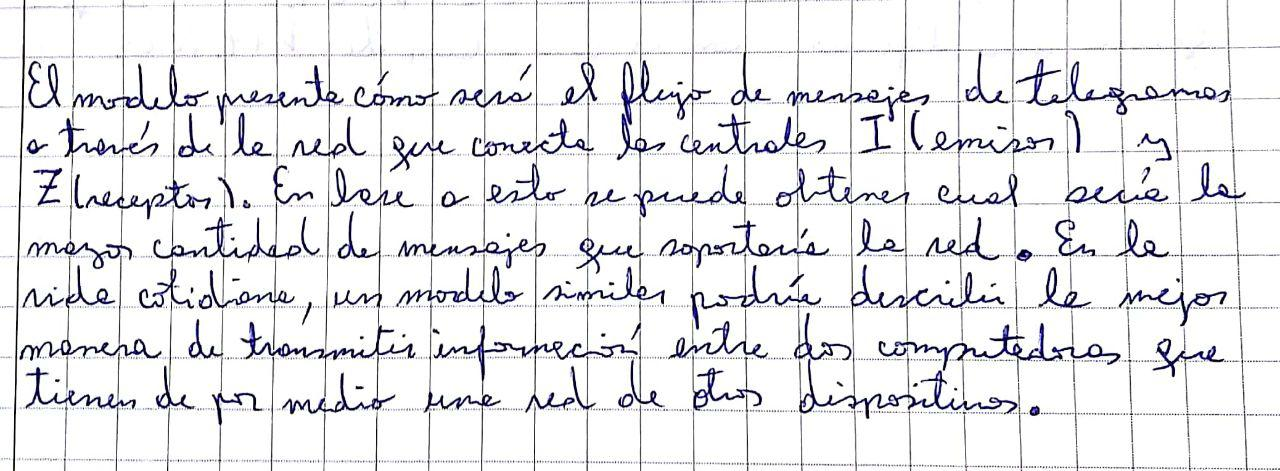
\includegraphics[scale=0.5]{claudio2.jpg}
	\caption*{Comentario de Claudio Durán}
\end{figure}
\begin{figure}[H]
	\centering
	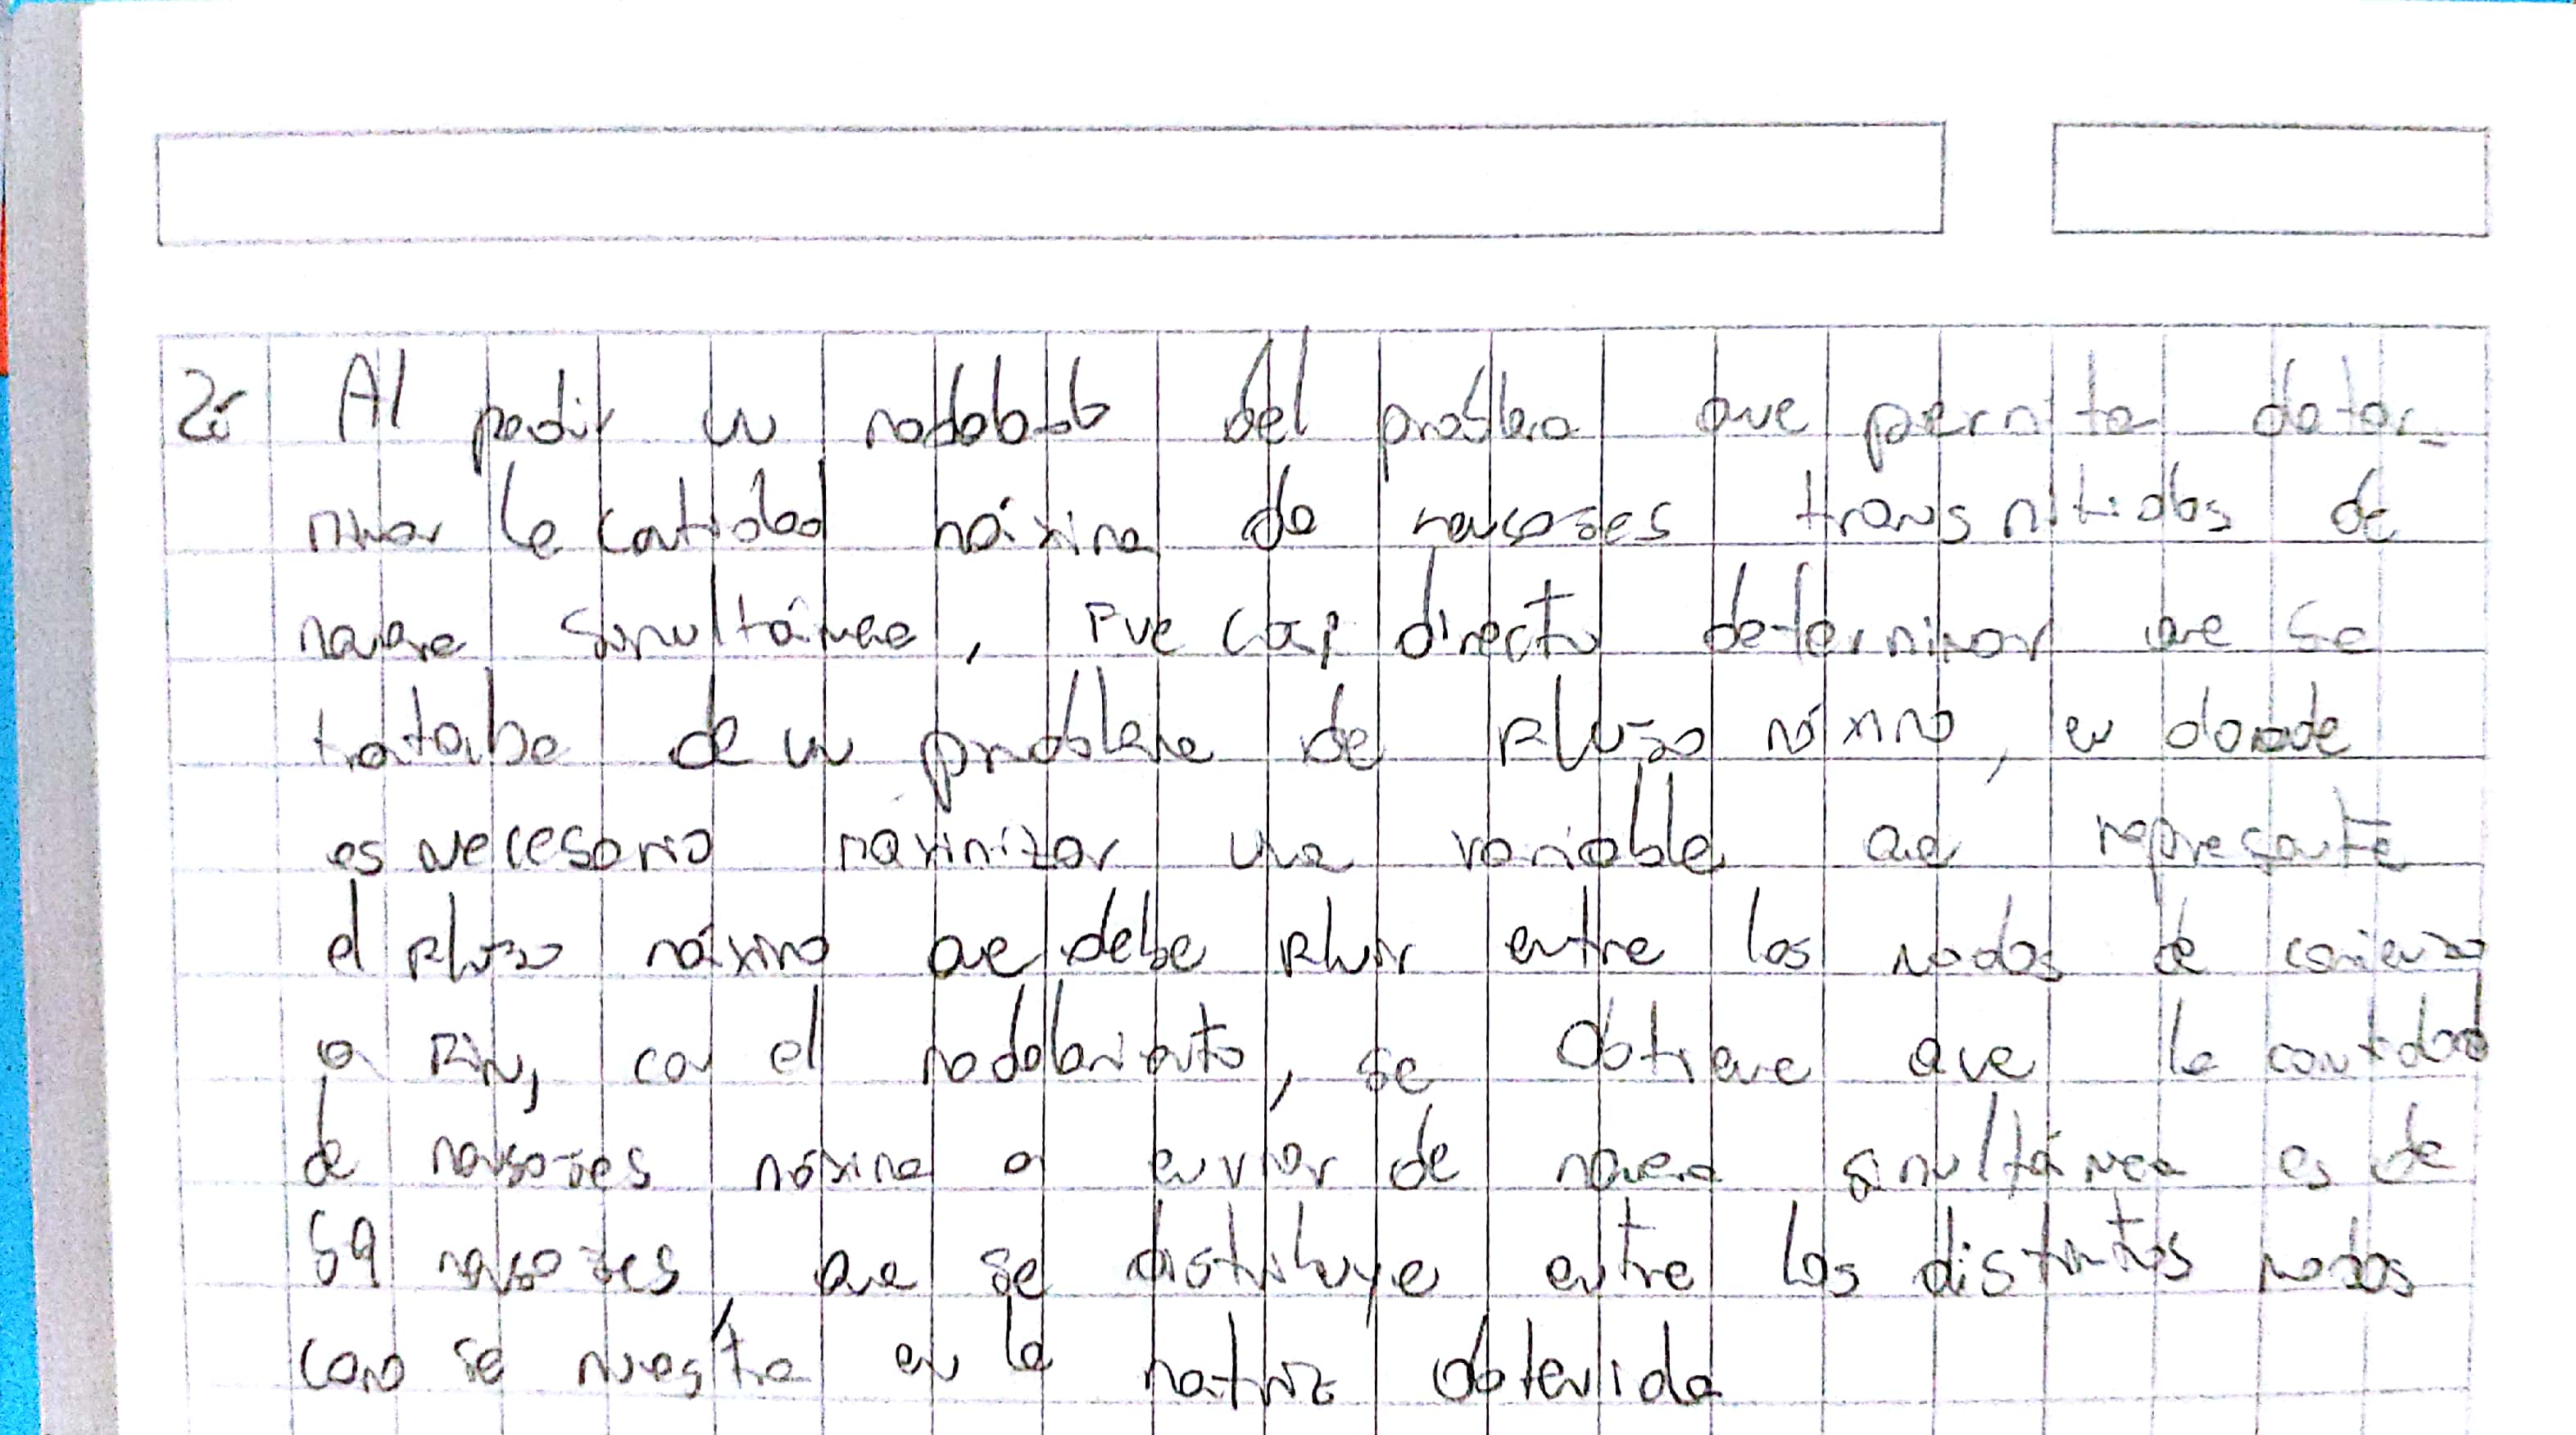
\includegraphics[scale=0.15]{martin2.jpg}
	\caption*{Comentario de Martin Mancilla}
\end{figure}
\newpage
\section{Tercer Problema}
\subsection{Formule  el  modelo  que  permita  construir  las  plantas de  tratamiento  de  aguas  servidas  al  mínimo  costo  asumiendo  que  cada  sitio  tiene  capacidad  ilimitada para  recibir  aguas  servidas  y  que  cada  área  de  recolección debe ser atendida únicamente por una planta}
\subsubsection{Constantes}
\begin{equation*}
\begin{split}
	A&=\{1,2,3,4,5,6,7,8,9,10\}\\
	B&=\{1,2,3,4,5,6,7\}\\
	Costo &= \begin{bmatrix}
	14 & 16 & 10 & 8 & 14 & 10 & 16\\
	12 & 11 & 12 & 14 & 14 & 12 & 14\\
	13 & 8 & 9 & 11 & 13 & 15 & 12\\
	10 & 15 & 14 & 12 & 16 & 15 & 13\\
	8 & 12 & 10 & 11 & 12 & 13 & 14\\
	11 & 10 & 8 & 6 & 11 & 8 & 9\\
	13 & 18 & 9 & 9 & 13 & 11 & 15\\
	15 & 12 & 11 & 14 & 12 & 16 & 10\\
	10 & 11 & 18 & 17 & 9 & 14 & 9\\
	9 & 16 & 13 & 12 & 10 & 8 & 8
	\end{bmatrix}\\
	CostoOP&=[8,10,9,11,9,10,12]\\
	CostoFijo&=[1000,800,700,1200,950,1150]\\
	MArea&=[500,700,1500,1000,1800,1200,1500,1000,900,1600]
\end{split}
\end{equation*}
\subsubsection{Variables de Decisión}
\begin{equation*}
\begin{split}
	X_j&=1 \text{; Si se utiliza sitio }j\quad \forall j \in B\\
	X_j&=0 \text{; En otro caso}\\\\
	Y_{ij}&=1 \text{; Área } i \text{ es atendida por sitio }j\quad \forall i \in A \wedge \forall j \in B\\
	Y_{ij}&=0 \text{; En otro caso}
\end{split}
\end{equation*}
\subsubsection{Función Objetivo}
\begin{equation*}
\begin{split}
	minZ&=\sum_{j=1}^{7}X_j\times CostoFijo[j]+\sum_{i=1}^{10}MArea[i]\sum_{j=1}^{7}Costo[i][j]\times Y_{ij}\\
	&+\sum_{j=1}^{7}CostoOP[j]\sum_{i=1}^{10}Y_{ij}\times MArea[i] \quad 
\end{split}
\end{equation*}
\subsubsection{Restricciones}
\begin{equation*}
	\begin{split}
		\text{(1) }&\sum_{j=1}^{7}Y_{ij}=1\quad \forall i\in A\\
		\text{(2) }&\sum_{j=1}^{7}Y_{ij}\leq 10\times X_{ij}\quad \forall j\in B\\
		\text{(3) }&X_{ij}\in\{0,1\}\forall i\in A \wedge \forall j\in B
	\end{split}
\end{equation*}
\subsubsection{Valores óptimos y solución}
\begin{itemize}
	\item Soluciones óptimas: $Y_{ij}=
	\begin{bmatrix}
	0 & 0 & 1 & 0 & 0 & 0 & 0\\
	1 & 0 & 0 & 0 & 0 & 0 & 0\\
	0 & 0 & 1 & 0 & 0 & 0 & 0\\
	1 & 0 & 0 & 0 & 0 & 0 & 0\\
	1 & 0 & 0 & 0 & 0 & 0 & 0\\
	0 & 0 & 1 & 0 & 0 & 0 & 0\\
	0 & 0 & 1 & 0 & 0 & 0 & 0\\
	0 & 0 & 1 & 0 & 0 & 0 & 0\\
	1 & 0 & 0 & 0 & 0 & 0 & 0\\
	1 & 0 & 0 & 0 & 0 & 0 & 0
	\end{bmatrix}$\\
	
	$X_{j}=
	\begin{bmatrix}
	1 & 0 & 1 & 0 & 0 & 0 & 0\\
	\end{bmatrix}$
	\item Valor óptimo = \$ 209800
\end{itemize}
\subsection{Formule  el  modelo  que  permita  construir  las  plantas  de  tratamiento  de  aguas  servidas  al  mínimo  costo, sabiendo que cada sitio puede  tratar a lo más 2.000 mirialitros mensuales y cada área de recolección debe ser atendida por una única planta}
Basta con agregar una restricción además del modelado creado para la parte anterior, junto a las demás restricciones:
\begin{equation*}
	\sum_{i=1}^{10}MArea[i]\times Y_{ij}\leq 2000\times X_j \quad \forall j \in B
\end{equation*}
\subsubsection{Valores óptimos y solución}
\begin{itemize}
	\item Soluciones óptimas: $Y_{ij}=
	\begin{bmatrix}
	0 & 0 & 0 & 1 & 0 & 0 & 0\\
	0 & 0 & 0 & 0 & 1 & 0 & 0\\
	0 & 1 & 0 & 0 & 0 & 0 & 0\\
	0 & 0 & 0 & 0 & 0 & 0 & 1\\
	1 & 0 & 0 & 0 & 0 & 0 & 0\\
	0 & 0 & 0 & 1 & 0 & 0 & 0\\
	0 & 0 & 1 & 0 & 0 & 0 & 0\\
	0 & 0 & 0 & 0 & 0 & 0 & 1\\
	0 & 0 & 0 & 0 & 1 & 0 & 0\\
	0 & 0 & 0 & 0 & 0 & 1 & 0
	\end{bmatrix}$
	\\
	$X_{j}=
	\begin{bmatrix}
	1 & 1 & 1 & 1 & 1 & 1 & 1\\
	\end{bmatrix}$
	\item Valor óptimo = \$ 227500
\end{itemize}
\subsection{Formule  el  modelo  que  permita  construir  las  plantas de  tratamiento  de  aguas  servidas  al  mínimo  costo, asumiendo  que  cada  sitio  tiene  capacidad  ilimitada de  recibir  aguas  servidas  y  que  cada  área  de  recolección puede enviar las aguas servidas a diferentes plantas de tratamiento}
\subsubsection{Constantes}
\begin{equation*}
\begin{split}
A&=\{1,2,3,4,5,6,7,8,9,10\}\\
B&=\{1,2,3,4,5,6,7\}\\
Costo &= \begin{bmatrix}
14 & 16 & 10 & 8 & 14 & 10 & 16\\
12 & 11 & 12 & 14 & 14 & 12 & 14\\
13 & 8 & 9 & 11 & 13 & 15 & 12\\
10 & 15 & 14 & 12 & 16 & 15 & 13\\
8 & 12 & 10 & 11 & 12 & 13 & 14\\
11 & 10 & 8 & 6 & 11 & 8 & 9\\
13 & 18 & 9 & 9 & 13 & 11 & 15\\
15 & 12 & 11 & 14 & 12 & 16 & 10\\
10 & 11 & 18 & 17 & 9 & 14 & 9\\
9 & 16 & 13 & 12 & 10 & 8 & 8
\end{bmatrix}\\
CostoOP&=[8,10,9,11,9,10,12]\\
CostoFijo&=[1000,800,700,1200,950,1150]\\
MArea&=[500,700,1500,1000,1800,1200,1500,1000,900,1600]
\end{split}
\end{equation*}
\subsubsection{Variables de Decisión}
\begin{equation*}
\begin{split}
	X_{ij}&=\text{ Cantidad enviada desde área } i \text{ a sitio } j\\
	\\
	Y_j&=1 \text{; Si se utiliza el sitio } j\\
	Y_j&=0 \text{; En otro caso}
\end{split}
\end{equation*}
\subsubsection{Función Objetivo}
\begin{equation*}
\begin{split}
	minZ &= \sum_{j=1}^{7}Y_j\times CostoFijo[j] + \sum_{j=1}^{7}\sum_{i=1}^{10}Costo[i][j]\times X_{ij}\\ 
	&+ \sum_{j=1}^{7}\sum_{i=1}^{10}CostoOP[j]\times X_{ij}
\end{split}
\end{equation*}
\subsubsection{Restricciones}
\begin{equation*}
\begin{split}
	\text{(1) }& \sum_{i=1}^{10}X_{ij}\leq Y_{j}\times \sum_{i=1}^{10}MArea[i]\quad\forall j\in B\\
	\text{(2) }&\sum_{j=1}^{7}X_{ij}=MArea[i]\quad\forall i\in A
\end{split}
\end{equation*}
\subsubsection{Valores óptimos y solución}
\begin{itemize}
	\item Soluciones óptimas: $X_{ij}=
	\begin{bmatrix}
	0 & 0 & 500 & 0 & 0 & 0 & 0\\
	700 & 0 & 0 & 0 & 0 & 0 & 0\\
	0 & 0 & 1500 & 0 & 0 & 0 & 0\\
	1000 & 0 & 0 & 0 & 0 & 0 & 0\\
	1800 & 0 & 0 & 0 & 0 & 0 & 0\\
	0 & 0 & 1200 & 0 & 0 & 0 & 0\\
	0 & 0 & 1500 & 0 & 0 & 0 & 0\\
	0 & 0 & 1000 & 0 & 0 & 0 & 0\\
	900 & 0 & 0 & 0 & 0 & 0 & 0\\
	1600 & 0 & 0 & 0 & 0 & 0 & 0
	\end{bmatrix}$
	\\
	$Y_{j}=
	\begin{bmatrix}
	1 & 0 & 1 & 0 & 0 & 0 & 0\\
	\end{bmatrix}$
	\item Valor óptimo = \$ 209800
\end{itemize}
\subsection{Formule  el  modelo  que  permita  construir  las  plantas de  tratamiento  de  aguas  servidas  al  mínimo  costo, asumiendo  que  cada  área  de  recolección  debe  ser  atendida  únicamente  por  una  planta  y  que  puede  ser construida solo una planta de tratamiento con capacidad ilimitada para recibir aguas servidas}
\subsubsection{Constantes}
\begin{equation*}
\begin{split}
A&=\{1,2,3,4,5,6,7,8,9,10\}\\
B&=\{1,2,3,4,5,6,7\}\\
Costo &= \begin{bmatrix}
14 & 16 & 10 & 8 & 14 & 10 & 16\\
12 & 11 & 12 & 14 & 14 & 12 & 14\\
13 & 8 & 9 & 11 & 13 & 15 & 12\\
10 & 15 & 14 & 12 & 16 & 15 & 13\\
8 & 12 & 10 & 11 & 12 & 13 & 14\\
11 & 10 & 8 & 6 & 11 & 8 & 9\\
13 & 18 & 9 & 9 & 13 & 11 & 15\\
15 & 12 & 11 & 14 & 12 & 16 & 10\\
10 & 11 & 18 & 17 & 9 & 14 & 9\\
9 & 16 & 13 & 12 & 10 & 8 & 8
\end{bmatrix}\\
CostoOP&=[8,10,9,11,9,10,12]\\
CostoFijo&=[1000,800,700,1200,950,1150]\\
MArea&=[500,700,1500,1000,1800,1200,1500,1000,900,1600]
\end{split}
\end{equation*}
\subsubsection{Variables de Decisión}
\begin{equation*}
\begin{split}
	Y_j&=1\text{; Si se utiliza sitio } j\quad \forall j \in B\\
	Y_{j}&= 0 \text{; En otro caso}\quad \forall j \in B
\end{split}
\end{equation*}
\subsubsection{Función Objetivo}
\begin{equation*}
\begin{split}
minZ &= \sum_{j=1}^{7}Y_j\times CostoFijo[j] + \sum_{i=1}^{10}MArea[i]\times \sum_{j=1}^{7} Costo[i][j]\times Y_j\\ 
&+ \sum_{i=1}^{10}MArea[i]\times\sum_{j=1}^{7} CostoOP[j]\times Y_j
\end{split}
\end{equation*}
\subsubsection{Restricciones}
\begin{equation*}
	\text{(1) }\sum_{j=1}^{7}Y_j=1
\end{equation*}
\subsubsection{Valores óptimos y solución}
\begin{itemize}
	\item Soluciones óptimas:
	$Y_{j}=
	\begin{bmatrix}
	1 & 0 & 0 & 0 & 0 & 0 & 0\\
	\end{bmatrix}$
	\item Valor óptimo = \$ 225000
\end{itemize}
\newpage
\subsection{Comentarios}
\begin{figure}[H]
	\centering
	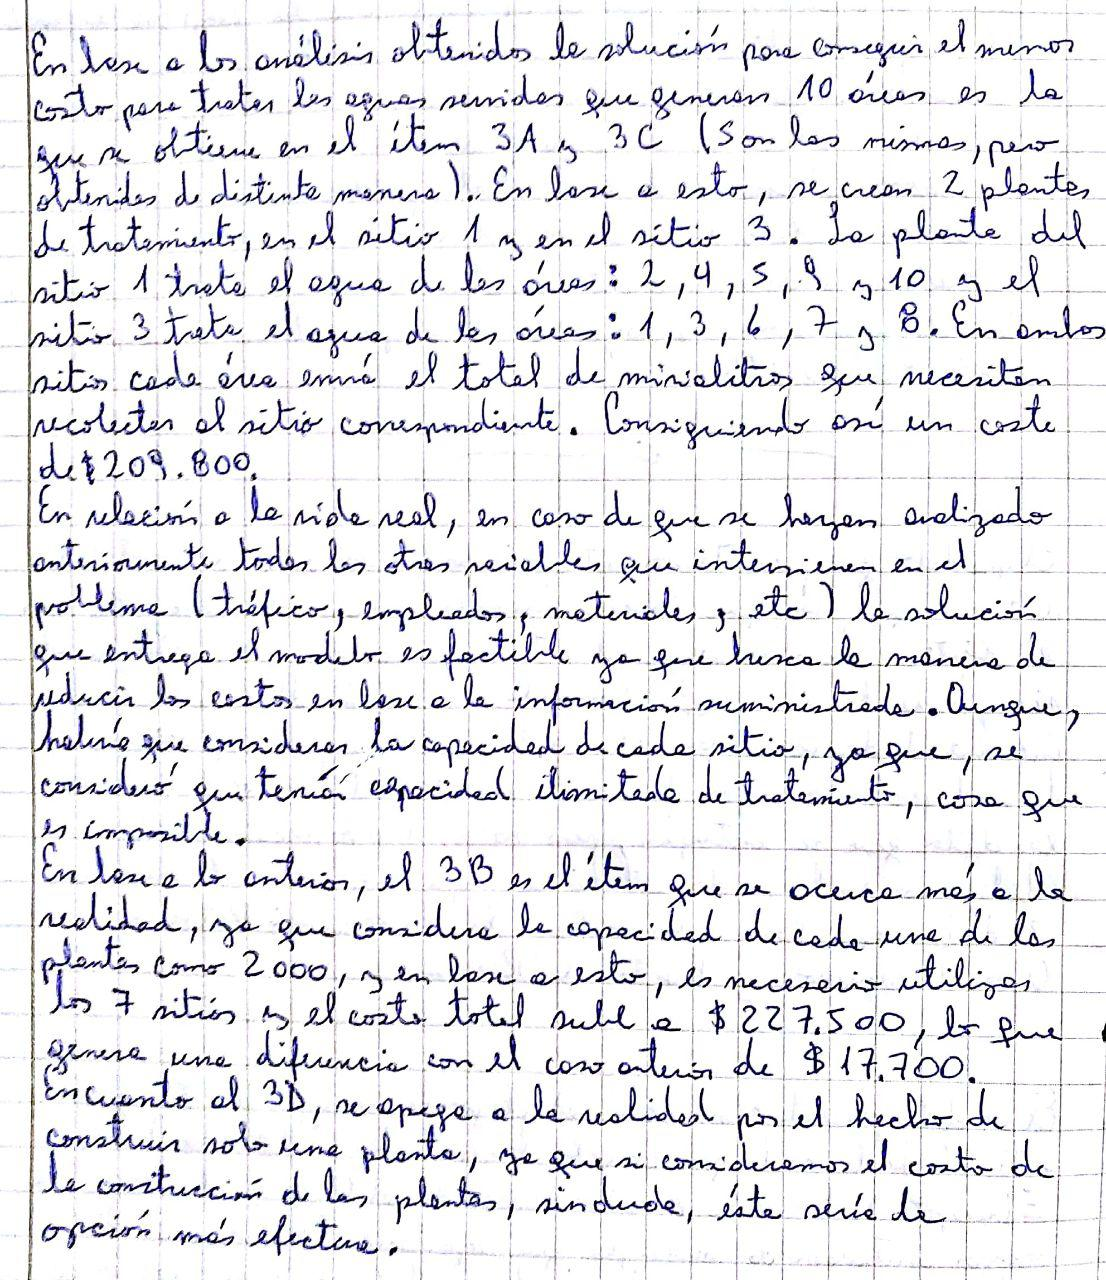
\includegraphics[scale=0.55]{claudio3.jpg}
	\caption*{Comentario de Claudio Durán}
\end{figure}
\begin{figure}[H]
	\centering
	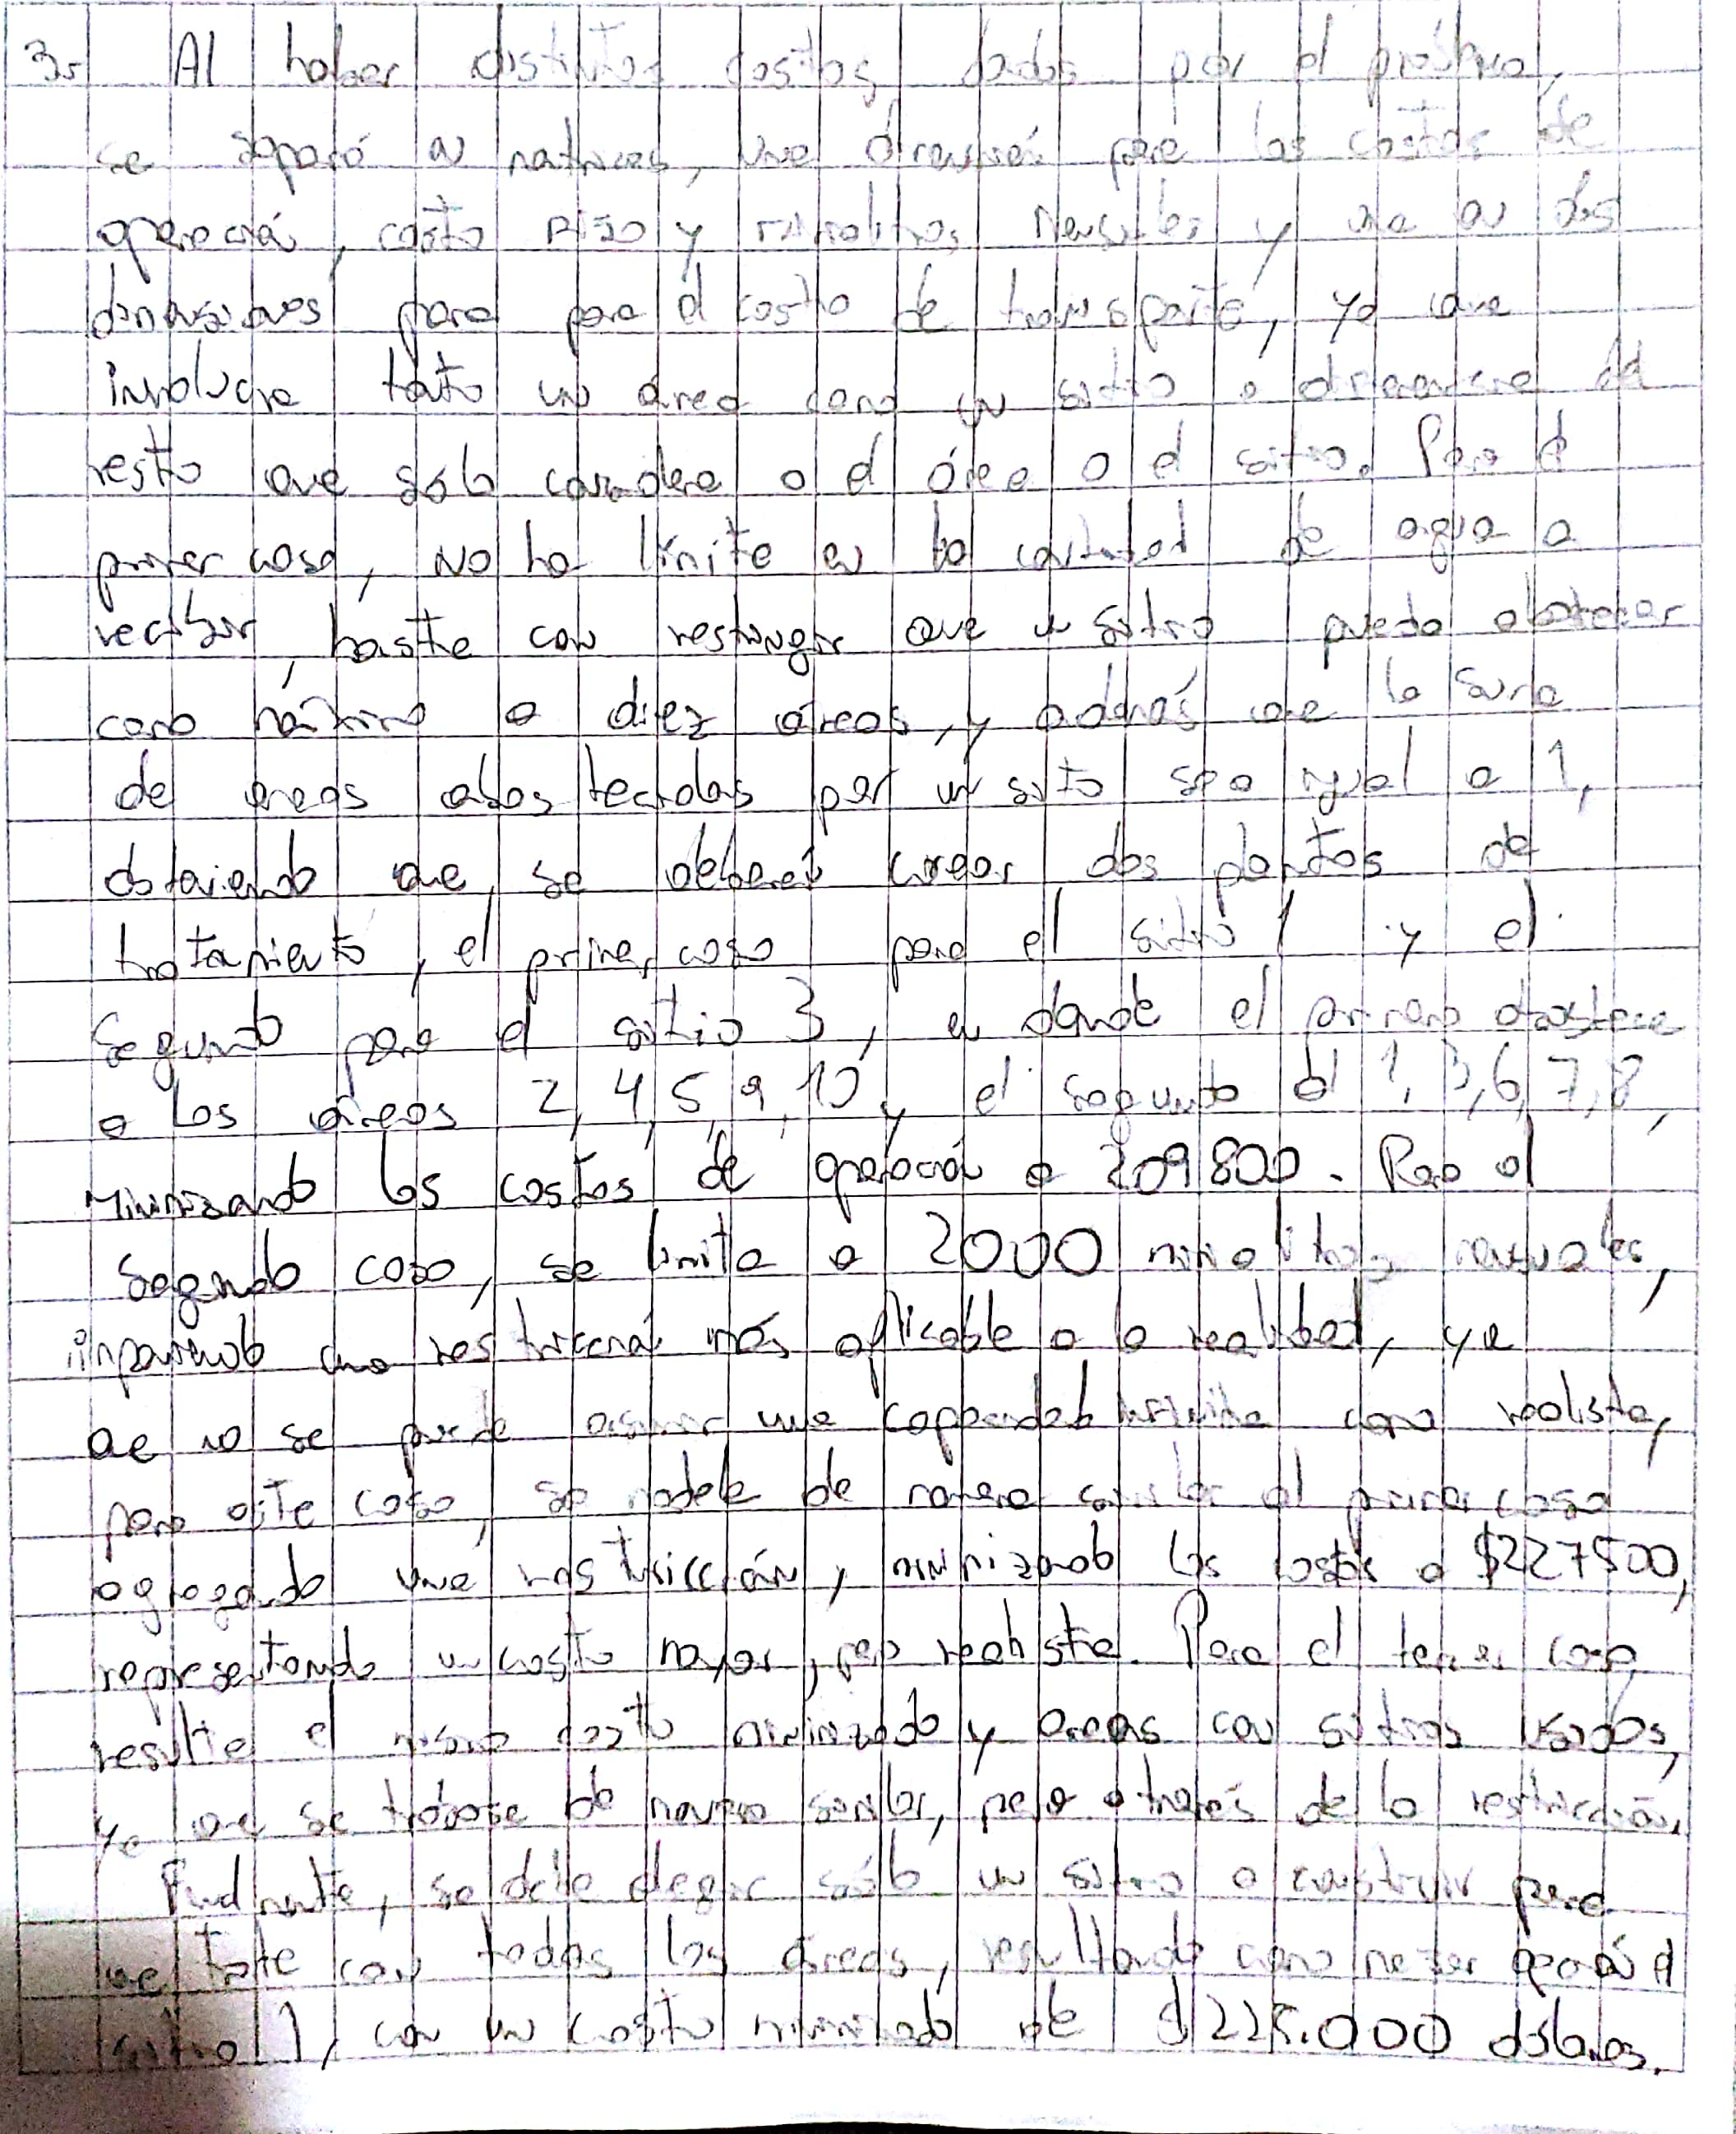
\includegraphics[scale=0.2]{martin3.jpg}
	\caption*{Comentario de Martin Mancilla}
\end{figure}
\end{document}